\documentclass{article}
\usepackage[utf8]{inputenc}
\usepackage{graphicx}
\usepackage{amsmath}

\title{Intelligens Fejlesztőeszkozok - 3. beadandó}
\author{Sándor Burian}
\date{Szeptember 2022}

\begin{document}

\maketitle

\section{feladat}

Az első egyenlet Euler plotja mindhárom lépésközzel:

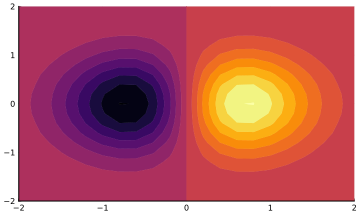
\includegraphics[scale=1]{../plot_3.png} 

A második egyenlet Euler plotja mindhárom lépésközzel:

\includegraphics[scale=1]{../plot_4.png} 

A harmadik egyenlet Euler plotjai mindhárom lépésközzel:

\includegraphics[scale=1]{../plot_5.png} 

\includegraphics[scale=1]{../plot_7.png} 

\includegraphics[scale=1]{../plot_8.png} 

3D plotok

\includegraphics[scale=1]{../plot_1.png} 

\includegraphics[scale=1]{../plot_2.png}

\includegraphics[scale=1]{../plot_6.png} 
 
\section{feladat}
Az első egyenlet RK2 plotja mindhárom lépésközzel:

\includegraphics[scale=1]{../plot_9.png} 

A második egyenlet RK2 plotja mindhárom lépésközzel:

\includegraphics[scale=1]{../plot_5.png} 

\section{feladat}
Az első feladat RK4 plotja mindhárom lépésközzel

\includegraphics[scale=1]{../plot_11.png} 

A második feladat RK4 plotja mindhárom lépésközzel

\includegraphics[scale=1]{../plot_10.png} 

\section{feladat}

A fenti ábrákból egyértelmúen látszik, hogy a megnövelt lépésköz pontatlanságot ad illetve jelentős torzítást. Továbbá látszik, hogy az Euler módszer nagyobb hibával ad eredményt mint az RK módszerek.

\includegraphics[scale=1]{../plot_13.png} 

\includegraphics[scale=1]{../plot_14.png} 

\includegraphics[scale=1]{../plot_15.png} 

\includegraphics[scale=1]{../plot_16.png} 

\includegraphics[scale=1]{../plot_17.png} 

\includegraphics[scale=1]{../plot_18.png} 

 
\end{document}
